\chapter{Protocolo de enrutamiento propuesto}
%-----------------------------------
%   PROTOCOLO DE ENRUTAMIENTO PROPUESTO
%-----------------------------------
\label{ch:protocolo_de_enrutamiento_propuesto}

Para que un enrutador pueda decidir hacia dónde retransmitir un paquete,
necesariamente debe tener información sobre sus vecinos. Por esta razón, todos
los protocolos de enrutamiento definen mensajes que los enrutadores transmiten
para intercambiar información entre ellos que les permita tomar estas
decidiones.

En el protocolo propuesto, cada vehículo y \textit{host}, una vez que tiene
cofngiurada su dirección IPv6, transmite mensajes para anunciar su presencia y
su ubicación ante los vecinos. De este modo, cuando un \textit{host} necesita
enviar un paquete a otro, puede seleccionar un vehículo vecino para que este se
encargue de enrutarlo. Del mismo modo, un vehículo que tenga que enrutar un
paquete, puede seleccionar el siguiente salto en la ruta.

En este capítulo, se decriben los tipos de mensajes que comparten los vehículos
y \textit{hosts}, y cómo se utilizan, junto con la información de la topología
vial, para realizar el enrutamiento de paquetes. 

\section{Criterios generales de retransmisión de paquetes}
%-----------------------------------
%   CRITERIOS GENERALES DE RETRANSMISIÓN DE PAQUETES
%-----------------------------------
\label{sec:criterios_generales_retransmision_paquetes}

Los protocolos basados en la posición, como se mencionó en la sección
\ref{sec:enrutamiento_basado_en_la_posicion}, consideran la ubicación de los
dispositivos para tomar decisiones sobre el enrutamiento. Por ejemplo, en el
protocolo GPSR, discutido en la sección \ref{subsubsec:retransmision_voraz},
cada nodo únicamente considera su ubicación, la del destinatario y las de los
vecinos, y selecciona el más cercano al destino como siguiente salto. Sin
embargo, en un entorno urbano es frecuente que existan obstáculos, como
edificios, que pueden bloquear las transmisiones. Este tipo de transmisiones se
conocen como \textbf{transmisiones sin línea de visión}. La figura
\ref{fig:transmision_sin_linea_de_vision} muestra una transmisión en la que un
edificio se encuentra entre los vehículos A y B.

\begin{figure}[th]
\centering
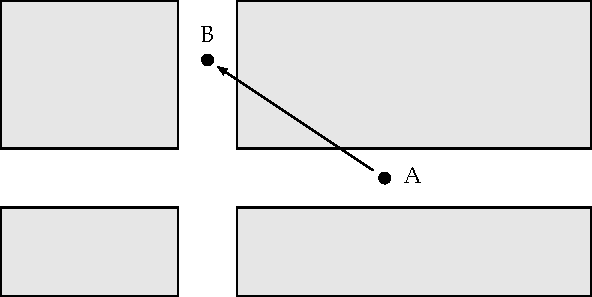
\includegraphics{transmision_sin_linea_de_vision}
\decoRule
\caption[Transmisión sin línea de visión]{Transmisión sin línea de visión.}
\label{fig:transmision_sin_linea_de_vision}
\end{figure}

Una transmisión sin línea de visión tiene alta posibilidad de provocar la
pérdida de un paquete, y cuando un paquete se pierde, debe ser retransmitido en
la mayoría de los casos. Si se pierden paquetes frecuentemente, la capacidad del
canal de comunicación comienza a utilizarse más para retransmitir paquetes
perdidos en vez de paquetes nuevos, y, como el canal inalámbrico es compartido
por todos los dispositivos, se generan cuellos de botella que causan pérdidas de
paquetes en las colas de paquetes de los enrutadores \cite{Kurose2013}.

Para reducir la pérdida de paquetes, el protocolo prupuesto busca que la mayoría
de las transmisiones entre los vehículos tengan línea de visión. Por ejemplo, en
la figura \ref{fig:transmision_misma_calle}, el vehículo A tiene un paquete cuya
ruta requiere que pase por C. Para esto, hay dos opciones para seleccionar el
siguiente salto: el vehículo B o directamente el vehículo C. Si se selecciona
C, la transmisión encontraría un edificio en el camino. Por otro lado, como A y
B tienen línea de visión, se seleccionaría B como siguiente salto, y después
este seleccionaría a C como siguiente salto.

\begin{figure}[th]
\centering
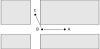
\includegraphics{transmision_misma_calle}
\decoRule
\caption[Transmisiones con línea de visión]{Transmisiones con línea de visión.}
\label{fig:transmision_misma_calle}
\end{figure}

En la figura\ref{fig:paquete_recorre_calle_1}, se muestra un paquete que es
retransmitido entre varios vehículos a lo largo de una ruta. En la figura
\ref{fig:paquete_recorre_calle_2}, se muestra el mismo escenario, pero a un
nivel de abstracción más alto, en el que se considera que el paquete recorre las
calles mediante las retransmisiones entre vehículos. Para lograr que los
vehículos retransmitan los paquetes de esta manera, cada vehículo debe conocer
la topología vial de la región Geohash donde se encuentra, y saber en qué calles
circulan sus vecinos.

\begin{figure}[th]
\centering
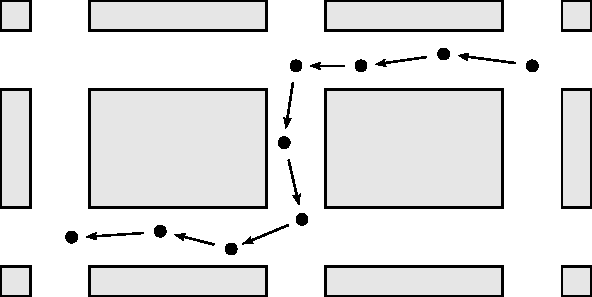
\includegraphics{paquete_recorre_calle_1}
\decoRule
\caption[Paquete siendo retransmitido entr vehículos]{Paquete siendo
retransmitido entre vehículos.}
\label{fig:paquete_recorre_calle_1}
\end{figure}

\begin{figure}[th]
\centering
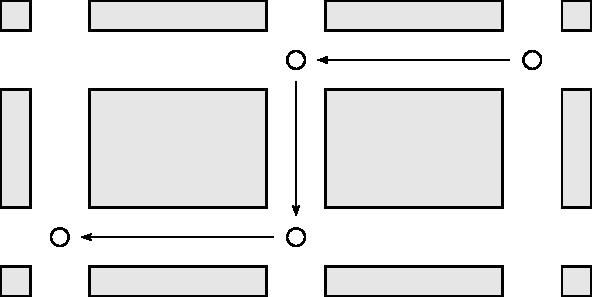
\includegraphics{paquete_recorre_calle_2}
\decoRule
\caption[Paquete recorriendo las calles]{Paquete recorriendo las calles.}
\label{fig:paquete_recorre_calle_2}
\end{figure}

\section{Base de datos de redes viales}
%-----------------------------------
%   BASE DE DATOS DE REDES VIALES
%-----------------------------------
\label{sec:base_de_datos_deredes_viales}

Una \textbf{red vial} es un grafo que representa una aproximación de la
topología vial de una región Geohash. Se trata de un grafo no dirigido
$\mathbf{G}=(\mathbf{V},\mathbf{E})$ en el que $\mathbf{V}$ es el conjunto de
vértices (cuya ubicación es conocida), que representan los cruces viales, y
$\mathbf{E}$ es el conjunto de aristas, que representan los segmentos de las
calles. La figura \ref{fig:red_vial_1} muestra el mapa de una región Geohash, y
su correspondiente grafo vial se muestra en la figura \ref{fig:red_vial_2}.

\begin{figure}[th!]
\centering
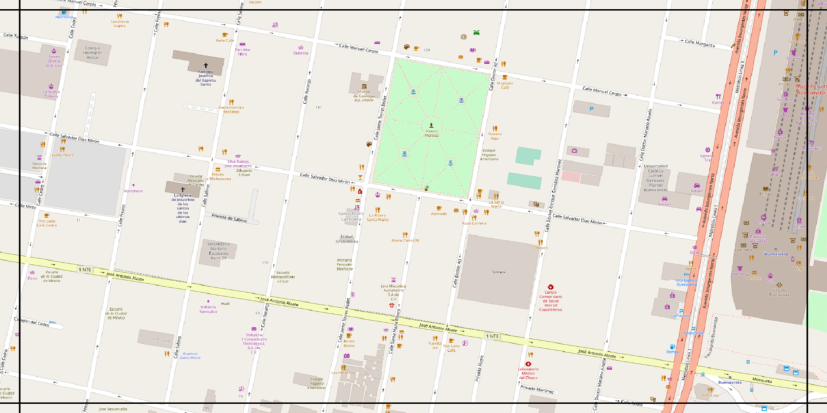
\includegraphics{grafo_vial_1} 
\decoRule
\caption[Región Geohash 9g3qxs]{Región Geohash 9g3qxs.}
\label{fig:red_vial_1}
\end{figure}

\begin{figure}[th!]
\centering
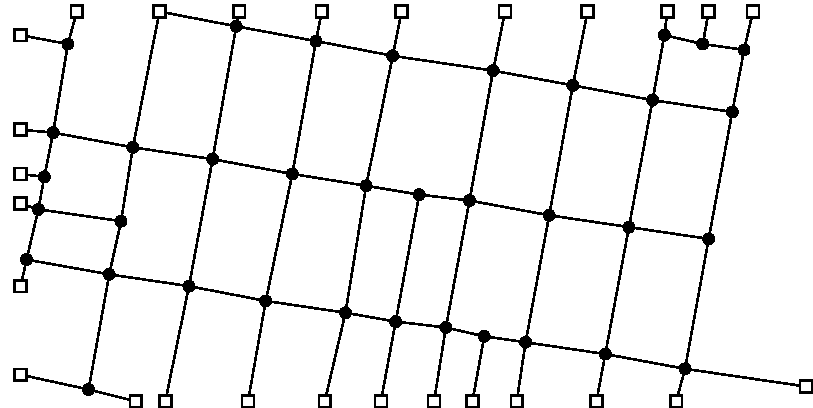
\includegraphics{grafo_vial_2} 
\decoRule
\caption[Red vial de la región Geohash 9g3qxs]{Red vial de la región
Geohash 9g3qxs.}
\label{fig:red_vial_2}
\end{figure}

Debido a que los vehículos están constantemente en movimiento, si se lograra
determinar una ruta que especifique por qué vehículos debe pasar un paquete para
llegar a su destino, esta tendría un tiempo de validez muy corto, ya que
probablemente algunos de los enlaces entre estos vehículos se romperían al poco
tiempo. En su lugar, se utilizan las redes viales para determinar las rutas, ya
que estas no cambian. Estas rutas indican las calles por las que debe pasar un
paquete para llegar a su destino, y se denominan \textbf{rutas viales}.

Una red vial no pretende ser una representación fiel de la infraestructura vial
física, sino que se usa como guía para determinar una ruta vial. Cada arista
representa todos los carriles que corresponden al segmento de calle que
representa, y cada vértice representa una ubicación en la que un vehículo puede
hacer una transmisión son posible línea de visión, no exclusivamente los cruces
viales.

Los vértices que se encuentran en el borde de una región, se muestran como
cuadrados en la figura \ref{fig:red_vial_2}. Estos se denominan \textbf{vértices
\textit{gateway}}, y son los que conectan las redes viales de dos regiones
adyacentes. De manera similar, las aristas que tienen un vértice
\textit{gateway} se denominan aristas \textit{gateway}. Con esto, el concepto
de región \textit{gateway} introducido en la sección \ref{sec:cambio_subred} se
redefine de la siguiente manera: un vehículo está en una región \textit{gateway}
si se encuentra en una arista \textit{gateway}.

Si un vehículo no conoce la red vial, es incapaz de calcular rutas viales. Es
por esto que cada vehículo debe contar \textit{a priori} con una \textbf{base de
datos de redes viales}, donde pueda consultar las redes viales de diferentes
regiones Geohash. Si un vehículo no conoce la red vial de una región, no puede
participar en el enrutamiento.

\section{Enrutamiento vial}
%-----------------------------------
%   ENRUTAMIENTO VIAL
%-----------------------------------
\label{sec:enrutamiento_vial}

Una ruta vial es una secuencia de aristas que une dos vértices dentro de una
misma red vial, y es independiente de la ubicación de los \textit{hosts} de
origen y destino. Por esta razón, no basta con conocer la ubicación del
\textit{host} de destino, sino que se necesita determinar un vértice de origen
y un vértice de destino para calcular una ruta vial. El vértice de destino de la
ruta se denomina \textbf{vértice de destino local}, ya que es el último vértice
por el que el paquete debe pasar para poder llegar al \textit{host} de destino.

Cuando un paquete está en la misma subred que su \textit{host} de destino, el
vértice de destino local es uno de los dos vértices de la arista en la que se
encuentra este \textit{host}. En la figura \ref{fig:enrutamiento_intrarregion},
el vehículo $V$ debe enrutar un paquete hacia el \textit{host} $D$, que se
encuentra en la misma subred. En este caso, se determina que el vértice de
destino local es $j$, y la ruta hacia este es $h \rightarrow g \rightarrow f
\rightarrow j$. Esta ruta se denomina \textbf{ruta intrarregión}.

\begin{figure}[th!]
\centering
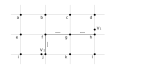
\includegraphics{enrutamiento_intrarregion}
\decoRule
\caption[Enrutamiento intrarregión]{Enrutamiento intrarregión.}
\label{fig:enrutamiento_intrarregion}
\end{figure}

Cuando un paquete se encuentra en una subred diferente a la subred en la que se
enuentra su \textit{host} de destino, este tiene que pasar por varias subredes
hasta llegar a la subred en la que se encuentra su destino. En la figura
\ref{fig:enrutamiento_interregion} el \textit{host} $S$ le tiene que enviar un
paquete al \textit{host} $D$, por lo que este tiene que pasar por las subredes
9g3qxu $\rightarrow$ 9g3qxs $\rightarrow$ 9g3qxt $\rightarrow$ 9g3qxm. Esta se
conoce como una \textbf{ruta intrarregión}.

\begin{figure}[th!]
\centering
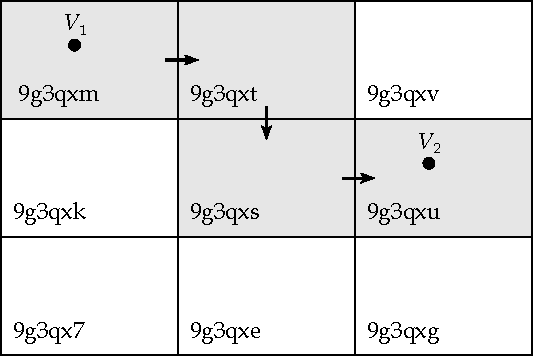
\includegraphics{enrutamiento_interregion}
\decoRule
\caption[Enrutamiento interregión]{Enrutamiento interregión.}
\label{fig:enrutamiento_interregion}
\end{figure}

Para que un paquete pueda pasar de una subred a otra, este debe llegar a un
vértice \textit{gateway}, y ahí se retransmite hacia la siguiente subred. En
este caso, dicho vértice \textit{gateway} es el vértice de destino local. En la
figura \ref{fig:enrutamiento_interregion_2}, el vehículo $V$ en la subred 1
tiene que enrutar un paquete hacia el \textit{host} $D$ en la subred 2.
Para esto, primero se busca una ruta hacia el vértice \textit{gateway} $h$ (que
se convierte en el vértice de destino local debido a su adyacencia con la
subred 2) y se enruta hacia este. La ruta que se obtiene es $e
\rightarrow j \rightarrow i \rightarrow h$. Una vez que el paquete se encuentra
en la subred 2, se calculará un nuevo vértice de destino local cerca del
\textit{host} $D$, y se enrutará hacia este.


\begin{figure}[th!]
\centering
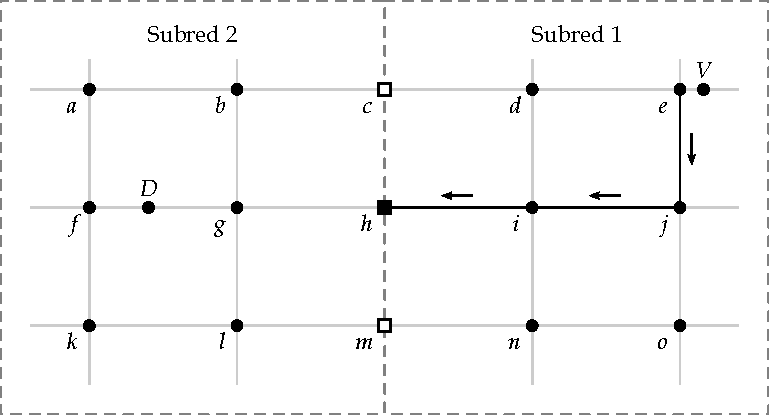
\includegraphics{enrutamiento_interregion_2}
\decoRule
\caption[Vértice de destino local en enrutamiento interregión]{Vértice de
destino local en enrutamiento interregión.}
\label{fig:enrutamiento_interregion_2}
\end{figure}

\section{Ubicación vial}
%-----------------------------------
%   UBICACIÓN VIAL
%-----------------------------------
\label{sec:ubicacion_vial}

Las rutas viales únicamente contienen información sobre la ubicación geográfica
de las calles o los vehículos, sino sobre la topología vial. Es por esto que los
vehículos necesitan conocer su ubicación respecto a la red vial y la de sus
vecinos para poder decidir cuál será el siguiente salto en la ruta vial.

Para este protocolo, se requiere que los dispositivos cuenten con un dispositivo
de geolocalización integrado, como se comentó en el capítulo
\ref{ch:protocolo_autoconfiguracion_de_direcciones_propuesto}. Cuando un
vehículo obtiene su ubicación geográfica, necesita conocer su ubicación dentro
de la red vial, que se conoce como \textbf{ubicación vial}.

La ubicación vial indica en qué arista de la red vial se encuentra un vehículo,
y su distancia a uno de los vértices de esta. Como la ubicación de los vértices
es conocida, a partir de su ubicación geográfica un vehículo puede calcular su
ubicación vial.

La figura \ref{fig:ubicacion_vial} muestra la ubicación vial del vehículo $V$,
que indica que se encuentra en la arista $(f,g)$, a una distancia $d$ del
vértice $f$.

\begin{figure}[th!]
\centering
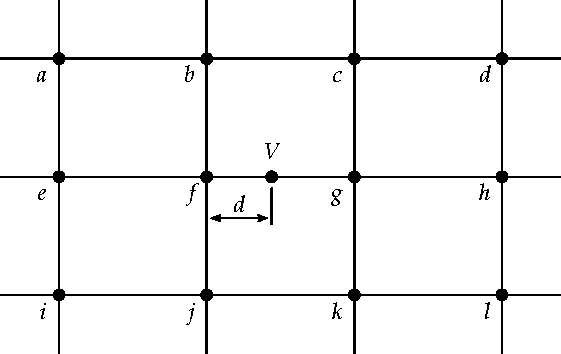
\includegraphics{ubicacion_vial} 
\decoRule
\caption[Ubicación vial de un vehículo]{Ubicación vial de un vehículo.}
\label{fig:ubicacion_vial}
\end{figure}

\section{Cabecera de opciones de salto por salto}
%-----------------------------------
%   CABECERAS DE OPCIONDES DE SALTO POR SALTO
%-----------------------------------
\label{sec:cabecera_opciones}

Los paquetes a enrutar deben incluir información que permita a los vehículos
decidir hacia dónde deben ser retransmitidos. Para esto, en el protocolo IPv6 se
especificanalgunos tipos de cabeceras llamadas cabeceras de extensión, que
sirven justamente para agregar información adicional a los datagramas. La
\keyword{cabecera de opciones de salto por salto} es una cabecera de extensión
cuya función es contener información que cada enrutador (vehículo en este caso)
que reciba el datagrama pueda revisar y modificar.Por esta razón, se usa esta
cabecera para incluir la información de enrutamiento en los paquetes.

La figura \ref{fig:formato_datagrama_ipv6_cabecera} muestra la estructura de un
datagrama IPv6 con la cabecera de opciones de salto por salto. El formato de
esta cabecera de extensión se muestra en la figura
\ref{fig:formato_cabecera_salto_por_salto} \cite{RFC2460}.

\begin{figure}[th!]
\centering
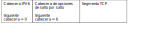
\includegraphics{formato_datagrama_ipv6_cabecera} 
\decoRule
\caption[Datagrama IPv6 con la cabecera de opciones de salto por
salto]{Datagrama IPv6 con la cabecera de opciones de salto por salto.}
\label{fig:formato_datagrama_ipv6_cabecera}
\end{figure}

\begin{figure}[th!]
\centering
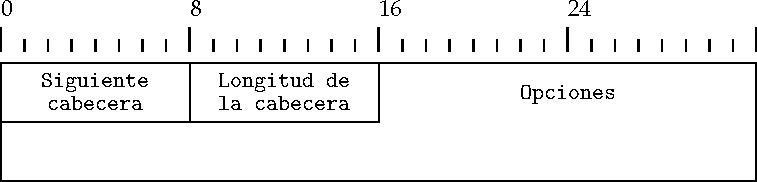
\includegraphics{formato_cabecera_salto_por_salto}
\decoRule
\caption[Formato de la cabecera de salto por salto]{Formato de la cabecera de
salto por salto.}
\label{fig:formato_cabecera_salto_por_salto}
\end{figure}

Los campos de la cabecera de opciones de salto por salto son los siguientes:

\keyword{Siguiente cabecera (8 bits)} -- Identifica el tipo de cabecera que
sigue después.

\keyword{Longitud de la cabecera (8 bits)} -- Longitud, en unidades de 8
octetos, de la cabecera de salto por salto, sin incluir los primeros 8 bytes.

\keyword{Opciones (longitud variable)} -- Secuencia de opciones que se procesan
en cada enrutador. Su longitud debe ser tal que la longitud total de la
cabecera de salto por salto sea un múltiplo entero de 8 octetos.

Las opciones se codifican con el formato tipo-longitud-valor (TLV), que se
muestra en la figura \ref{fig:formato_tlv}. Los campos de cada opción son los
siguientes \cite{RFC2460}:

\begin{figure}[th!]
\centering
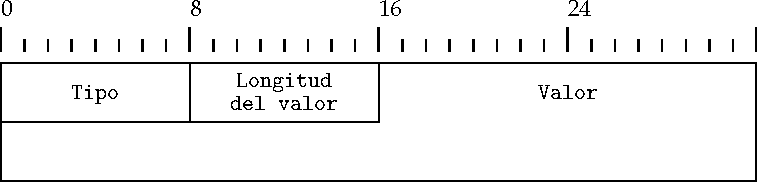
\includegraphics{formato_tlv}
\decoRule
\caption[Formato TLV]{Formato TLV.}
\label{fig:formato_tlv}
\end{figure}

\keyword{Tipo (8 bits)} -- Identificador del tipo de opción.

\keyword{Longitud del valor (8 bits)} -- Longitud en octetos del campo del
valor del dato.

\keyword{Valor (longitud variable)} -- Valor de la opción.

En el tipo de opción, los dos primeros bits indican qué hacer si la opción no
es reconocida, y el tercer bit indica si el valor del dato puede cambiar o no a
lo largo de la ruta.

A continuación, se describen las opciones que incluye la cabecera de opciones de
salto por salto de los datagramas que los vehículos deben enrutar.

\subsection{Opción de ubicación del destino}
%-----------------------------------
%   OPCIÓN DE UBICACIÓN DEL DESTINO
%-----------------------------------
\label{subsec:opcion_de_ubicacion_del_destino}

Para poder enrutar un paquete, el \textit{host} que lo origina agrega la
\keyword{opción de ubicación del destino} a la cabecera de opciones de salto
por salto. El formato de la opción de ubicación del destino se muestra en la
figura \ref{fig:formato_opcion_ubicacion_destino}, y contiene los siguientes
campos:

\begin{figure}[th!]
\centering
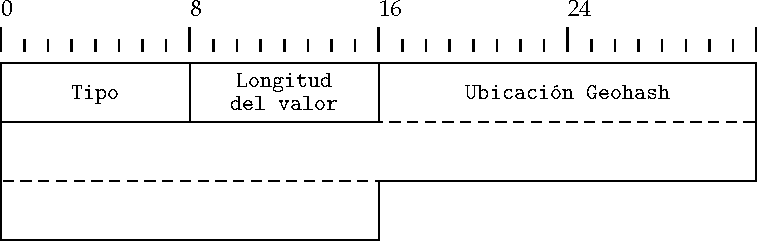
\includegraphics{formato_opcion_ubicacion_destino}
\decoRule
\caption[Formato de la opción de ubicación del destino]{Formato de la opción de
ubicación del destino.}
\label{fig:formato_opcion_ubicacion_destino}
\end{figure}

\keyword{Tipo (8 bits)} -- El tipo de la opción es 88, donde los primeros dos
bits indican que el paquete debe ser descartado si no se reconoce el tipo de
opción, y el tercer bit indica que el valor de la opción no cambia a lo largo
de la ruta.

\keyword{Longitud del valor (8 bits)} -- La longitud del valor es de 8 octetos.

\keyword{Ubicación Geohash (64 bits)} -- Ubicación Geohash de longitud 12 del
\textit{host} de destino.

\subsection{Opción de ubicación vial del destino}
%-----------------------------------
%   OPCIÓN DE UBICACIÓN VIAL DEL DESTINO
%-----------------------------------
\label{subsec:opcion_de_ubicacion_vial_del_destino}

Cuando un vehículo recibe un paquete, puede revisar la opción de ubicación del
destino para saber la ubicación geográfica a donde este tiene que llegar. Pero
para calcular una ruta vial hacia este, también se debe conocer la ubicación
vial destino.

Si un vehículo recibe un paquete cuyo destino se encuentra en la misma subred,
debe calcular la ubicación vial del destino y agregarla a la cabecera de
opciones con la \keyword{opción de ubicación vial del destino}. El formato de
este tipo de opción se muestra en la figura
\ref{fig:formato_opcion_ubicacion_vial_destino}, y contiene los siguientes
campos:

\begin{figure}[th!]
\centering
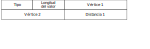
\includegraphics{formato_opcion_ubicacion_vial_destino}
\decoRule
\caption[Formato de la opción de ubicación vial del destino]{Formato de la
opción de ubicación vial del destino.}
\label{fig:formato_opcion_ubicacion_vial_destino}
\end{figure}

\keyword{Tipo (8 bits)} -- El tipo de la opción es 25, donde los primeros dos
bits indican que la opción se ignora si no se reconoce el tipo de opción, y el
tercer bit indica que el valor no cambia a lo largo de la ruta.

\keyword{Longitud del valor (8 bits)} -- La longitud del valor es de 6 octetos.

\keyword{Vértice 1 (16 bits)} -- Vértice 1 de la arista donde se ecuentra el
destino.

\keyword{Vértice 2 (16 bits)} -- Vértice 2 de la arista donde se ecuentra el
destino.

\keyword{Distancia 1 (16 bits)} -- Valor entero de la distancia en metros al
vértice 1.

Si un el destino un paquete se encuentra en una subred diferente a la subred en
la que este se encuentra, no necesita llevar esta opción, ya que primero debe
llegar a la subred correspondiente. El primer vehículo que recibe el paquete y
se encuentra en la misma subred que el \textit{host} de destino, se encarga de
agregar esta opción.

\subsection{Opción de vértices visitados}
%-----------------------------------
%   OPCIÓN DE VÉRTICES VISITADOS
%-----------------------------------
\label{subsec:opcion_de_vertices_visitados}

Para evitar que un paquete pase más de una vez por el mismo vértice, este debe
llevar un registro de los vértices por los que ya ha pasado. Estos se indican en
la \keyword{opción de vértices visitados}. El formato de esta opción se indica
en la figura \ref{fig:formato_opcion_vertices_visitados}, y contiene los
siguientes campos:

\begin{figure}[th!]
\centering
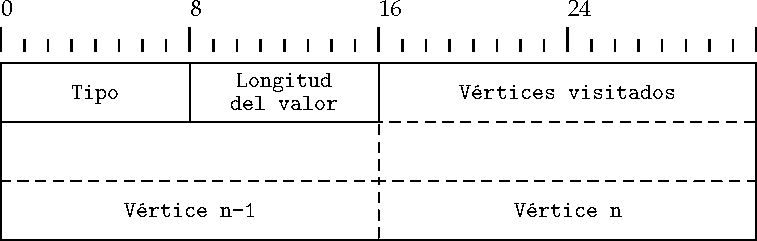
\includegraphics{formato_opcion_vertices_visitados}
\decoRule
\caption[Formato de la opción de vértices visitados]{Formato de la opción de
vértices visitados.}
\label{fig:formato_opcion_vertices_visitados}
\end{figure}

\keyword{Tipo (8 bits)} -- El tipo de la opción es 58, donde los primeros dos
bits indican que la opción se ignora si no se reconoce el tipo de opción, y el
tercer bit indica que el valor puede cambiar a lo largo de la ruta.

\keyword{Longitud del valor (8 bits)} -- La longitud del valor es variable.

\keyword{Vértices visitados (longitud variable)} -- Lista de vértices por los
que el paquete ha pasado. Cada vértice ocupa 2 octetos.

La opción de vértices visitados sólo es válida dentro de una subred. Cuando un
paquete pasa de una subred a otra, se elimina la opción de vértices visitados
de la cabecera y se agrega una nueva para los vértices de la siguiente subred.

\subsection{Verificación de la cabecera de opciones de salto por salto}
%-----------------------------------
%   VERIFICACIÓN DE LA CABECERA DE OPCIONES DE SALTO POR SALTO
%-----------------------------------
\label{subsec:verificacion_cabecera_opciones_salto_por_salto}

Para que un paquete pueda ser enrutado, lo mínimo que debe contener en su
cabecra de opciones de salto por salto es la opción de ubicación del destino, y
es responsabilidad del \textit{host} que emite el paquete garantizar que esta
opción esté presente. Si el paquete no contiene esta información, no hay manera
de saber hacia dónde se debe enrutar.

Si un vehículo recibe un paquete, primero verifica que tenga la opción de
ubicación del destino. De ser así, después se verifica si la ubicación del
destino está en su misma región. Si este es el caso, y el paquete no contiene la
opción de ubicación vial del destino, esta se calcula y se agrega a la cabecera
de opciones de salto por salto. Esta opción únicamente es necesaria cuando un
paquete se encuentra en la misma región que su destino.

Después, se verifica si el paquete incluye la opción de vértices visitados. Si
no es así, significa que el vehículo recibió el paquete directamente del
\textit{host} que lo emite, o que acaba de entrar a una nueva subred, por lo que
la opción los vértices visitados anterior no es válida para la nueva red vial,
por lo que se eliminó esta opción. En este caso, se agrega una nueva opción de
vértices visitados vacía al paquete.

\section{Mensajes de enrutamiento}
%-----------------------------------
%   FORMATO DE LOS MENSAJES
%-----------------------------------
\label{sec:mensajes_de_enrutamiento}

Como se mencionó anteriormente, los vehículos y \textit{hosts} necesitan
compartir entre sí información que les permita saber cuáles son sus vecinos y
dónde se encuentran, para así poder elegir el siguiente salto en luna ruta. A
continuación, se describe el formato de estos mensajes.

\subsection{Hola-vehículo (HOLA-VEHIC)}
%-----------------------------------
%   MENSAJE HOLA-VEHÍCULO
%-----------------------------------
\label{subsec:mensaje_hola_vehic}

El mensaje HOLA-VEHIC contiene la ubicación geográfica y la ubicación vial de un
vehículo, y tiene una longitud de 40 octetos. Su formato se muestra en la figura
\ref{fig:formato_hola_vehic}. Los campos del mensaje son los siguientes:

\begin{figure}[th!]
\centering
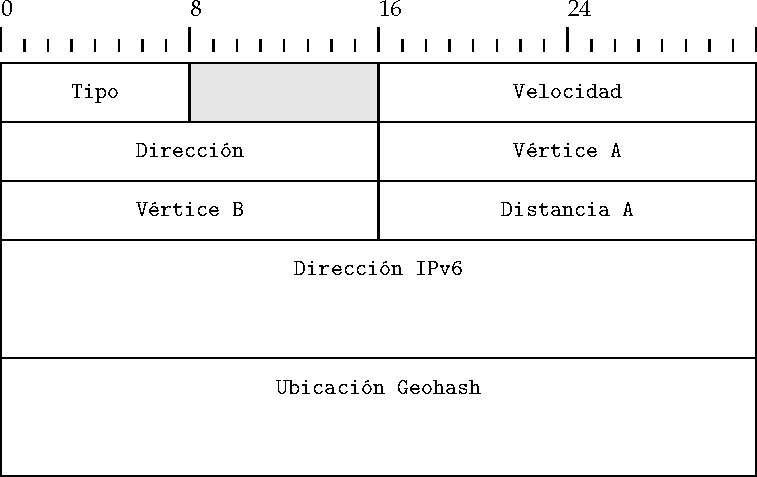
\includegraphics{formato_hola_vehic}
\decoRule
\caption[Formato del mensaje HOLA-VEHIC]{Formato del mensaje HOLA-VEHIC.}
\label{fig:formato_hola_vehic}
\end{figure}

\keyword{Tipo (8 bits)} -- Su valor es \code{1} para indicar que se trata de un
mensaje HOLA-VEHIC.

\keyword{Velocidad (16 bits)} -- Velocidad del vehículo en m/s.

\keyword{Dirección (16 bits)} -- Ángulo acimutal de la dirección del movimiento
del vehículo en grados.

\keyword{Vértice A (16 bits)} -- Primer vértice de la arista por la que
circula el vehículo.

\keyword{Vértice B (16 bits)} -- Segundo vértice de la arista por la que
circula el vehículo.

\keyword{Distancia A (16 bits)} -- Distancia en metros del vehículo al vértice
A.

\keyword{Dirección IPv6 (128 bits)} -- Dirección IPv6 del vehículo que
transmite el mensaje.

\keyword{Ubicación Geohash (64 bits)} -- Ubicación Geohash de longitud 12 del
vehículo al momento de transmitir el mensaje.

\subsection{Hola-\textit{host} (HOLA-HOST)}
%-----------------------------------
%   MENSAJE HOLA-HOST
%-----------------------------------
\label{subsec:mensaje_hola_host}

El mensaje HOLA-HOST contiene la ubicación geográfica de un \textit{host}, y
tiene una longitud de 28 octetos. Su formato se muestra en la figura
\ref{fig:formato_hola_host}. Los campos del mensaje son los siguientes:

\begin{figure}[th!]
\centering
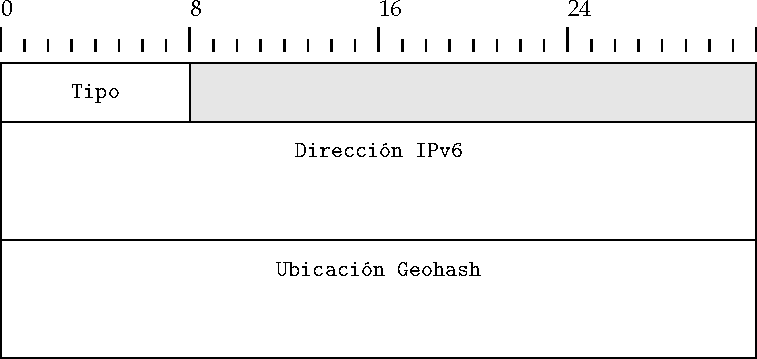
\includegraphics{formato_hola_host}
\decoRule
\caption[Formato del mensaje HOLA-HOST]{Formato del mensaje HOLA-HOST.}
\label{fig:formato_hola_host}
\end{figure}

\keyword{Tipo (8 bits)} -- Su valor es \code{2} para indicar que se trata de un
mensaje HOLA-HOST.

\keyword{Dirección IPv6 (128 bits)} -- Dirección del \textit{host} que emite el
mensaje.

\keyword{Ubicación Geohash (65 bits)} -- Ubicación Geohash del \textit{host} al
momento de transmitir el mensaje.

\section{Directorio de vehículos vecinos}
%-----------------------------------
%   DIRECTORIO DE VEHÍCULOS VECINOS
%-----------------------------------
\label{sec:directiorio_vehiculos_vecinos}

\begin{sloppypar}
Para que un vehículo pueda elegir el siguiente salto para un paquete, o para
que un \textit{host} pueda enviar un paquete, necesita saber cuáles son sus
vehículos vecinos y la ubicación de estos. Para esto, cada vehículo transmite
periódicamente mensajes \mbox{HOLA-VEHIC}, con los que anuncia su presencia
ante sus vecinos, e indica su ubicación geográfica y su ubicación vial. Estos
mensajes se transmiten a la dirección \textit{multicas} de la subred, y la
frecuencia con la que se transmiten se define por el parámetro de configuración
\mbox{INTERVALO\_HOLA\_VEHIC}.
\end{sloppypar}

\begin{sloppypar}
Cuando un vehículo o \textit{host} recibe un mensaje \mbox{HOLA-VEHIC} de un
vehículo vecino, se registra en el \keyword{directorio de vehículos vecinos}. De
este modo, puede saber qué vehículos están cerca y dónde se encuentran, y así
decidir cuál será el siguiente salto para un paquete.
\end{sloppypar}

\begin{sloppypar}
Cada registro en el directorio se identifica con la dirección IPv6 del vehículo
vecino, y tiene una vigencia definida por el parámetro de configuración
\mbox{VIGENCIA\_VEHICULO\_VECINO}. Si se recibe un mensaje \mbox{HOLA-VEHIC} y
ya existe un registro para la dirección del vehículo que lo emitió, se actualiza
el registro. Y si el tiempo de expiración de un registro se cumple, este se
elimina.
\end{sloppypar}

Los campos de cada registro son los siguientes:

\begin{center}
\begin{tabular}{ r l }
Dirección IP: & Tiempo de expiración \\
& Ubicación \\
& Velocidad \\
& Dirección de movimiento \\
& Vértice A \\
& Vértice B \\
& Distancia a A \\
& Distancia a B
\end{tabular}
\end{center}

\keyword{Tiempo de exporación} -- Tiempo hasta el que el registro es válido.

\keyword{Ubicación Geohash} -- Ubicación del vehículo.

\keyword{Velocidad} -- Velocidad del vehículo en m/s.

\keyword{Dirección del movimiento} -- Ángulo acimutal de la dirección del
movimiento del vehículo en grados.

\keyword{Vértice A} -- Primer vértice de la arista por la que
circula el vehículo. Es el vértice hacia el que se dirige el vehículo.

\keyword{Vértice B} -- Segundo vértice de la arista por la que
circula el vehículo.

\keyword{Distancia A} -- Distancia al vértice A.

\keyword{Distancia B} -- Distancia al vértice B.

\section{Directorio de \textit{hosts} vecinos}
%-----------------------------------
%   DIRECTORIO DE HOSTS VECINOS
%-----------------------------------
\label{sec:directorio_hosts_vecinos}

\begin{sloppypar}
Si un vehículo tiene un paquete dirigido a un \textit{host} que está a su
alcance, debe tener una manera de saberlo, por lo que los \textit{hosts} también
tienen que anunciar su presencia ante sus vehículos vecinos. Para esto,
transmiten periódicamente mensajes \mbox{HOLA-HOST} indicando su ubicación
geográfica, que también se transmiten a la dirección \textit{multicast} de la
subred, y la frecuencia con la que se transmiten se define por el parámetro de
configuración \mbox{INTERVALO\_HOLA\_HOST}.
\end{sloppypar}

\begin{sloppypar}
Cuando un vehículo recibe un mensaje \mbox{HOLA-HOST} de un \textit{host}
vecino, se registra en el \textbf{directorio de \textit{hosts} vecinos}. Así,
podrá saber si el destino de un paquete es un \textit{host} que está a su
alcance, y enviárselo directamente si este es el caso.
\end{sloppypar}

\begin{sloppypar}
Cada registro del directorio se identifica con la dirección IPv6 del
\textit{host} vecino, y tiene una vigencia definida por el parámetro de
configuración \mbox{VIGENCIA\_HOST\_VECINO}. Si se recibe un mensaje
\mbox{HOLA-HOST} y ya existe un registro para la dirección del \textit{host} que
lo emitió, se actualiza el registro. Y si el tiempo de expiración de un registro
se cumple, este se elimina.
\end{sloppypar}

Los campos de cada registro son los siguientes:

\begin{center}
\begin{tabular}{ r l }
Dirección IP: & Tiempo de expiración \\
& Ubicación \\
\end{tabular}
\end{center}

\keyword{Tiempo de exporación} -- Tiempo hasta el que el registro es válido.

\keyword{Ubicación} -- Ubicación del \textit{host}.

\section{Cómputo de rutas viales}
%-----------------------------------
%   CÓMPUTO DE RUTAS VIALES
%-----------------------------------
\label{sec:computo_rutas_viales}

En la figura \ref{fig:ruta_mala}, se muestra una ruta para ir del vértice $d$
al vértice $i$, en la que hay giros de ángulos considerables en cuatro esquinas.
Si un paquete siguiera esta ruta, las transmisiones podrían ser interferidas por
algúnun edificio en cada una de estas esquinas. Por otro lado, en la figura
\ref{fig:ruta_buena}, se muestra otra ruta equivalente, pero esta se forma por
dos tramos rectos largos de aristas, y sólo un giro en una esquina. Si un
paquete siguiera esta ruta, únicamente en una esquina las transmisiones
correrían riesgo de ser interferidas por algún edificio. Es por esto que,
para tratar de evitar la pérdida de paquetes, se busca que las rutas viales se
formen por tramos rectos lo más largos que sea posible.

\begin{figure}[th!]
\centering
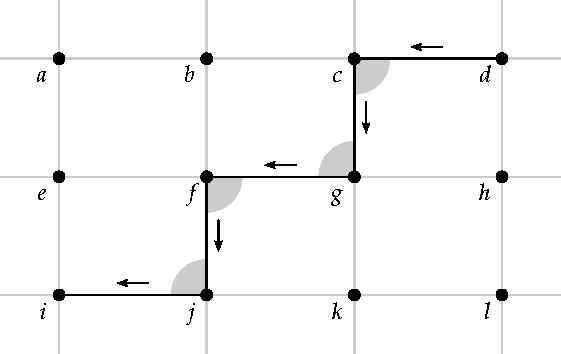
\includegraphics{ruta_mala}
\decoRule
\caption[Ruta con muchos tramos cortos de aristas]{Ruta con muchos tramos
cortos de aristas.}
\label{fig:ruta_mala}
\end{figure}

\begin{figure}[th!]
\centering
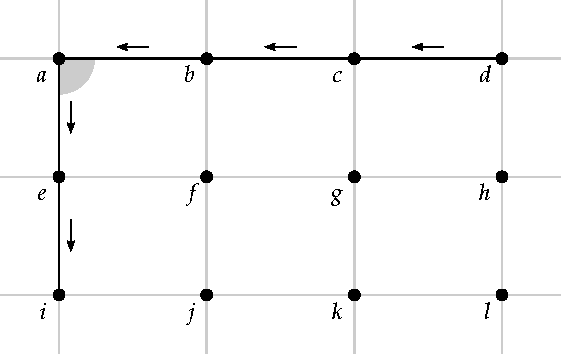
\includegraphics{ruta_buena}
\decoRule
\caption[Ruta con pocos tramos largos de aristas]{Ruta con pocos tramos largos
de aristas.}
\label{fig:ruta_buena}
\end{figure}

Para utilizar un algoritmo para determinar las rutas en la red vial, es
necesario asignar un peso a cada una de las aristas. Sin embargo, para
determinar las rutas con la consideración anterior, el peso de cada arista
depende de la arista anterior en la ruta. Por ejemplo, en la ruta de la figura
\ref{fig:ruta_mala}, para ir al vértice $g$ desde la arista $(d,c)$, hay un
giro de ángulo considerable, por lo que la arista $(c,g)$ tiene un peso grande
en esta ruta. En contraste, en la ruta de la figura \ref{fig:ruta_buena}, para
ir al vértice $b$ desde la arista $(d,c)$, el tramo es recto, por lo que la
arista $(c,b)$ tendrá un peso pequeño en esta ruta.

Existen algoritmos que calculan las rutas más cortas desde un vértice inicial al
resto de los vértices de un grafo, como el algoritmo de Dijkstra
\cite{cormen2001}. Sin embargo, este algoritmo requiere que todas las aristas
tengan un peso definido previamente. Es por esto que se propone un algoritmo
que calcula las rutas más cortas en la red vial inspirado en el algoritmo de
Dijkstra, pero con ciertas diferencias.

Por lo general, un vehículo no se encuentra en un vértice de la red vial, sino
en algún punto a lo largo de una arista. Por esta razón, el cálculo de las
rutas viales no comienza en un solo vértice, sino en los dos vértices de la
arista por la que circula el vehículo. Además de esto, los pesos de las aristas
se calculan conforme el algoritmo progresa, y su valor es igual al ángulo que
forma la dirección de la arista con su arista predecesora. Por ejemplo, en la
figura \ref{fig:calculo_pesos}, se inicia el cálculo de las rutas viales en la
arista $(g,h)$. Se puede observar que para ir desde esta arista a los vértices
$c$, $f$ y $k$, se debe hacer un giro de 90\si{\degree}, 0\si{\degree} y
90\si{\degree}, respectivamente, y estos serán sus pesos.

Otro punto a considerar es que un paquete pudo ya haber pasado por un conjunto
de vértices, lo que se pueden saber revisando la opción de vértices visitados
en la cabecera de opciones de salto por salto. Además, es posible que no existan
vehículos vecinos en alguna arista a los que transmitir paquetes, por lo que
estos datos también se consideran en el procedimiento del cálculo de la rutas.

\begin{figure}[th!]
\centering
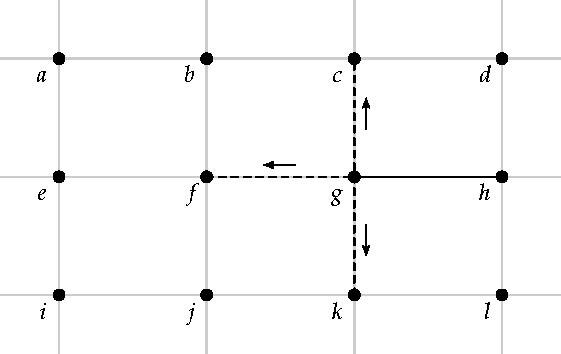
\includegraphics{calculo_pesos}
\decoRule
\caption[Cálculo de los pesos de las aristas]{Cálculo de los pesos de las
aristas.}
\label{fig:calculo_pesos}
\end{figure}

\begin{algorithm}[th!]
\small
\caption{Cálculo de la ruta más corta}
\label{alg:ruta_mas_corta}
\DontPrintSemicolon
\LinesNumbered
    \KwData{$\mathbf{G}$: Grafo vial, $(a,b)$: Arista inicial, $VV$: Conjunto
    de vértices visitados, $AE$: Conjunto de aristas disponibles}
    \Begin{
        \ForEach{$v \in \mathbf{G}.\mathbf{V}$} {
            $distancias[v] \gets \infty$ \;
        }
        $distancias[a] \gets 0$ \;
        $distancias[b] \gets 0$ \;
        $S \gets \mathbf{G.V} \setminus \{a,b\}$ \;
        \ForEach{$v \in \mathbf{G.V} \mid (a,v) \in \mathbf{G.E}$}{
            \If{$v \neq b$}{ \eIf{$v \notin VV$ y $(a,v) \in AE$}{
                    $distancias[v] \gets calcularPeso((a,v), (a,b))$ \;
                    $predecesores[v] \gets a$ \;
                }{
                    $S \gets S \setminus \{v\}$ \;
                }
            }
        }
        \ForEach{$v \in \mathbf{G.V} \mid (b,v) \in \mathbf{G.E}$}{
            \If{$v \neq a$}{
                \eIf{$v \notin VV$ y $(b,v) \in AE$}{
                    $peso \gets calcularPeso((b,v),(a,b)$) \;
                    \If{$peso < distancias[v]$}{
                        $distancias[v] \gets peso$ \;
                        $predecesores[v] \gets b$ \;
                    }
                }{
                    $S \gets S \setminus \{v\}$ \;
                }
            }
        }
        \While{$S \neq \emptyset$}{
            $v \gets$ vértice en $S$ con menor distancia \;
            $u \gets predecesores[v]$ \;
            \ForEach{$w \in \mathbf{G}.\mathbf{V}$ adyacente a $v$}{
                \If{$w \neq u$}{
                    \eIf{$w \notin VV$}{
                        $peso \gets calcularPeso((v,w),(u,v))$ \;
                        \If{$distancias[w] > distancias[v] + peso$}{
                            $distancias[w] \gets distancias[v] + peso$ \;
                            $predecesores[w] \gets v$ \;
                        }
                    }{
                        $S \gets S \setminus \{w\}$ \;
                    }
                }
            }
            $S \gets S \setminus \{v\}$ \;
        }
        \Return{predecesores, distancias}
    }
\end{algorithm}

El algoritmo \ref{alg:ruta_mas_corta} describe el procedimiento propuesto para
determinar las rutas en una red vial. Este recibe como datos de entrada la
la red vial $\mathbf{G}$, la arista inicial $(a,b)$, el conjunto $NV$ de
vértices visitados por el paquete, y el conjunto $NE$ de aristas disponibles.
Este algoritmo utiliza dos vectores principales cuyo tamaño es igual al número
de vértices en la red vial. El vector $predecesores$ contiene el vértice
predecesor de cada vértice a lo largo de la ruta. El vector $distancias$ indica
la \textbf{distancia de ruta} desde la arista inicial hasta cada uno de los
vértices, que es la suma de los pesos de todas las aristas hasta dicho
vértice. También utiliza el conjunto $S$, que contiene los vértices que faltan
por procesar.

En las líneas 2-5, se establece la distancia de ruta a cada vértice como
$\infty$, excepto para los vértices iniciales, cuya distancia de ruta es 0. En
la línea 6, se agregan todos los vértices a $S$, excepto los dos vértices de la
arista inicial. En las líneas 7-13, se calcula la distancia de ruta a los
vértices adyacentes a $a$, y se asigna este como predecesor (excepto para los
vértices visitados). En las líneas 14-22, se realiza el mismo procedimiento,
pero para los vértices adyacentes a $b$. Nótese que la distancia de ruta de los
vértices visitados nunca deja de ser $\infty$.

En las líneas 23-35, se calcula la ruta a cada uno de los vértices restantes.
Primero, se busca el vértice $v$ en $S$ cuya distancia de ruta sea la menor, y
su predecesor $u$. Después, para cada vértice $w$ adyacente a $v$, se calcula el
peso de la arista $(v,w)$ desde la arista $(u,v)$, y se actualiza la distancia a
$w$ si esta es menor al valor anterior. Finalmente, una vez que se calculó y
actualizó la distancia a cada uno de los vértices adyacentes a $v$, se elimina
$v$ de $S$, lo que significa que se terminó de procesar. El resultado final son
los vectores $predecesores$ y $distancias$.

Una vez calculadas las rutas viales al resto de los vértices, se determina la
mejor ruta para el paquete que se va a retransmitir. Si el destino se encuentra
en la misma región, se revisa su ubicación vial para saber en qué arista se
encuentra. Después, se revisa cuál de los dos vértices de esta arista tiene una
ruta de menor distancia y se selecciona como vértice de destino local.

Si el destino se encuentra en otra región, se verifica hacia qué dirección se
encuentra, y se obtienen los vértices \textit{gateway} en esta dirección.
Después, se busca entres estos el que tenga la menor distancia de ruta y se
selecciona como vértice de destino local. Por ejemplo, si la región en la que se
encuentra el destino se encuentra al sureste, se busca el vértice de destino
local entre los vértices \textit{gateway} al sur y al este. Si se encuentra al
norte, se busca sólo entre los vértices \textit{gateway} al norte.

\section{Selección del siguiente salto}
%-----------------------------------
%   SELECCIÓN DEL SIGUIENTE SALTO
%-----------------------------------
\label{sec:seleccion_siguiente_salto}

Una vez que se determina el vértice de destino local y se tiene una ruta hacia
este, se debe seleccionar el siguiente salto para retransmitir el paquete. El
objetivo de cada retransmisión es que el paquete haga el mayor avance posible en
la ruta, intentando que haya línea de visión con el siguiente salto.

Como se mencionó anteriormente, las rutas se forman por tramos rectos lo más
largos posible. Obteniendo el primer tramo recto en la ruta, se puede saber
cuál es el vehículo vecino que se encuentra más adelante en dicho tramo, y se
selecciona como siguiente salto. En la figura \ref{fig:siguiente_salto_1}, el
vehículo $V_0$ calculó una ruta para un paquete, en la que el primer tramo recto
es $j \rightarrow i \rightarrow h \rightarrow g \rightarrow f$. Este tiene en su
directorio de vehículos vecinos a los vehículos $V_1$, $V_2$ y $V_3$, pero sólo
$V_1$ y $V_2$ se están en el primer tramo recto de la ruta. De los dos, $V_2$ es
el que se encuentra más adelante en este tramo, por lo que se selecciona como
siguiente salto.

\begin{figure}[th!]
\centering
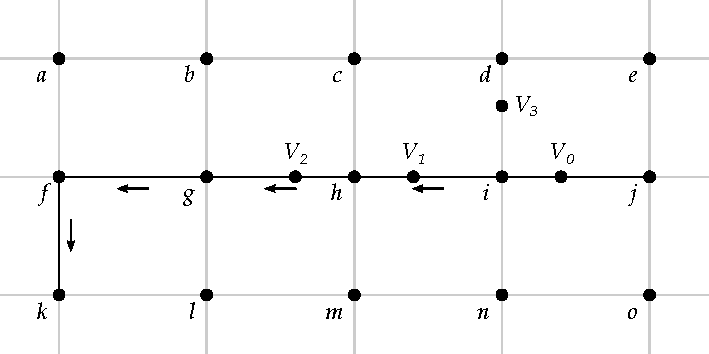
\includegraphics{siguiente_salto_1}
\decoRule
\caption[Siguiente salto en el primer tramo recto de la ruta]{Siguiente salto
en el primer tramo recto de la ruta.}
\label{fig:siguiente_salto_1}
\end{figure}

En caso de que no exista un vecino que se encuentre adelante en el primer tramo
recto, se obtiene el siguiente tramo recto, y se elige como siguiente salto el
vecino más cercano al inicio de este tramo. En la figura
\ref{fig:siguiente_salto_2}, el vehículo $V_0$ calculó una ruta para un
paquete, y el primer tramo recto es $i \rightarrow n$, pero no hay vehículos en
este. El siguiente tramo recto es $n \rightarrow m \rightarrow l \rightarrow
k$, y los vehículos $V_1$ y $V_2$ se encuentran en este tramo. El vecino más
cercano al inicio de este tramo es $V_1$, por lo que este se selecciona como
siguiente salto.

\begin{figure}[th!]
\centering
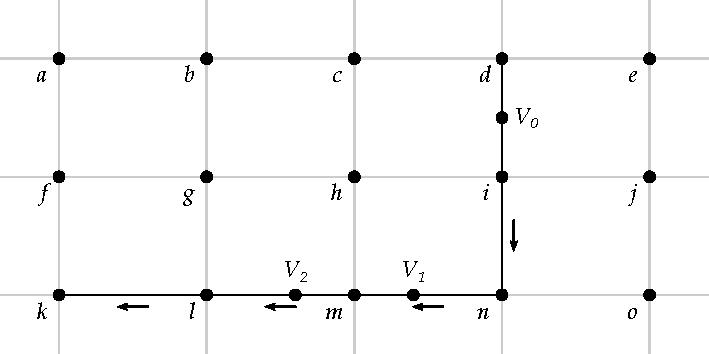
\includegraphics{siguiente_salto_2}
\decoRule
\caption[Siguiente salto en el segundo tramo recto de la ruta]{Siguiente salto
en el segundo tramo recto de la ruta.}
\label{fig:siguiente_salto_2}
\end{figure}

Cuando un vehículo se encuentra en una arista \textit{gateway} y tiene que
retransmitir un paquete hacia la subred adyacente, este selecciona el vehículo
vecino más cercano que se encuentre en la subred adyacente. Si no hay vecinos
en la subred adyacente, se selecciona como siguiente salto el vecino más
cercano al vértice \textit{gateway}. En la figura \ref{fig:siguiente_salto_3},
los vehículos $V_0$ y $V_1$ están en la subred 1, y los vehículos $V_2$ y $V_3$
en la subred 2. $V_0$ debe retransmitir un paquete hacia la subred 2, y como se
encuentra en la arista \textit{gateway} $(i,h)$, selecciona a $V_2$ como
siguiente salto, ya que es el vecino más cercano que se encuentra en la subred
adyacente. Si $V_2$ no estuviera en el directorio de vehículos vecinos de $V_0$,
este tendría que seleccionar a $V_1$ como siguiente salto, ya que es el vecino
más cercano al vértice \textit{gateway} $h$.

\begin{figure}[th!]
\centering
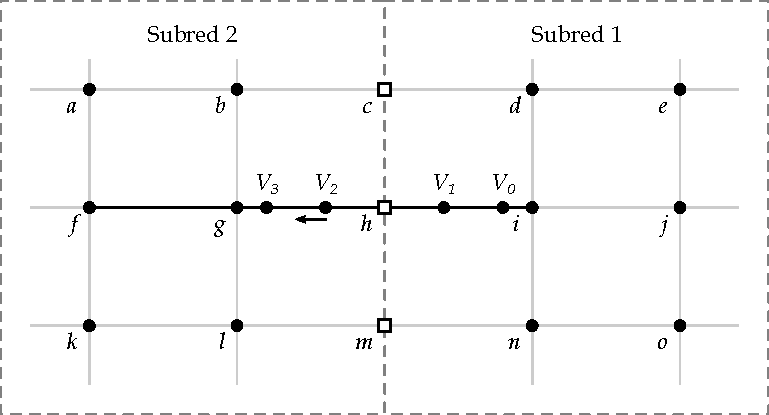
\includegraphics{siguiente_salto_3}
\decoRule
\caption[Siguiente salto al cambiar de subred]{Siguiente salto al cambiar de
subred.}
\label{fig:siguiente_salto_3}
\end{figure}

Para saber dónde termina un tramo recto de una ruta, se recorre vértice por
vértice, y mientras la distancia de ruta de cada vértice esté cerca de 0, se
considera que el tramo de la ruta hasta dicho vértice es un tramo recto. En la
figura \ref{fig:tramo_recto}, se muestra una ruta que inicia en la arista
$(j,i)$. La siguiente arista es $(i,h)$, y su peso es 0 (véase la sección
\ref{sec:computo_rutas_viales}), por lo que la distancia de ruta del vértice
$h$ es 0. Siguiendo el mismo análisis, la distancia de ruta de los vértices
$g$ y $f$ también son 0. Después, la siguiente arista es $(f,k)$, y su peso es
90, ya que esta forma un ángulo de 90\si{\degree} con la arista $(g,f)$, por lo
que la distancia de ruta del vértice $k$ es 90. Así, se determina que el primer
tramo recto de la arista termina en el vértice $f$.

\begin{figure}[th!]
\centering
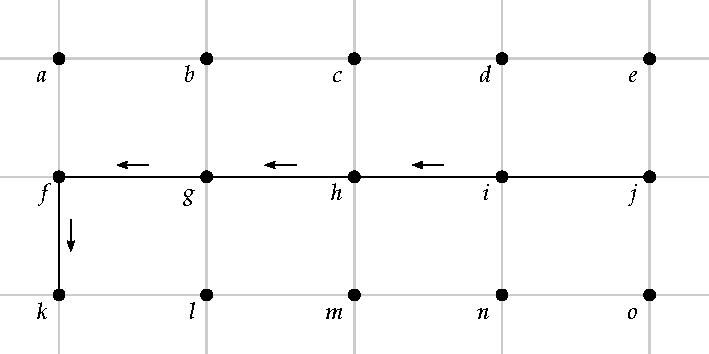
\includegraphics{tramo_recto}
\decoRule
\caption[Primer tramo recto de una ruta vial]{Primer tramo recto de una ruta
vial.}
\label{fig:tramo_recto}
\end{figure}

\section{Lista de parámetros de configuración}
%-----------------------------------
%   LISTA DE PARÁMETROS DE CONFIGURACIÓN
%-----------------------------------
\label{sec:lista_de_parametros_de_configuracion}

Los parámetros de configuración del protocolo de enrutamiento propuesto son los
siguientes:

\keyword{INTERVALO\_HOLA\_VEHIC} -- Intervalo de tiempo que cada vehículo espera
para transitir un mensaje HOLA-VEHIC.

\keyword{VIGENCIA\_VEHICULO\_VECINO} -- Tiempo de vigencia de cada registro del
directorio de vehículos vecinos a partir del último mensaje HOLA-VEHIC
correspondiente recibido.

\keyword{INTERVALO\_HOLA\_HOST} -- Intervalo de tiempo que cada \textit{host}
espera para transmitir un mensaje HOLA-HOST.

\keyword{VIGENCIA\_HOST\_VECINO} -- Tiempo de tiempo que cada registro del
directorio de \textit{hosts} vecinos a partir del último mensaje HOLA-HOST
correspondiente recibido.

\keyword{VIGENCIA\_RUTA} -- Tiempo de vigencia de cada ruta en la tabla de
enrutamiento.
